\documentclass[11pt,preprint, authoryear]{elsarticle}

\usepackage{lmodern}
%%%% My spacing
\usepackage{setspace}
\setstretch{1.2}
\DeclareMathSizes{12}{14}{10}{10}

% Wrap around which gives all figures included the [H] command, or places it "here". This can be tedious to code in Rmarkdown.
\usepackage{float}
\let\origfigure\figure
\let\endorigfigure\endfigure
\renewenvironment{figure}[1][2] {
    \expandafter\origfigure\expandafter[H]
} {
    \endorigfigure
}

\let\origtable\table
\let\endorigtable\endtable
\renewenvironment{table}[1][2] {
    \expandafter\origtable\expandafter[H]
} {
    \endorigtable
}


\usepackage{ifxetex,ifluatex}
\usepackage{fixltx2e} % provides \textsubscript
\ifnum 0\ifxetex 1\fi\ifluatex 1\fi=0 % if pdftex
  \usepackage[T1]{fontenc}
  \usepackage[utf8]{inputenc}
\else % if luatex or xelatex
  \ifxetex
    \usepackage{mathspec}
    \usepackage{xltxtra,xunicode}
  \else
    \usepackage{fontspec}
  \fi
  \defaultfontfeatures{Mapping=tex-text,Scale=MatchLowercase}
  \newcommand{\euro}{€}
\fi

\usepackage{amssymb, amsmath, amsthm, amsfonts}

\def\bibsection{\section*{References}} %%% Make "References" appear before bibliography


\usepackage[round]{natbib}

\usepackage{longtable}
\usepackage[margin=2.3cm,bottom=2cm,top=2.5cm, includefoot]{geometry}
\usepackage{fancyhdr}
\usepackage[bottom, hang, flushmargin]{footmisc}
\usepackage{graphicx}
\numberwithin{equation}{section}
\numberwithin{figure}{section}
\numberwithin{table}{section}
\setlength{\parindent}{0cm}
\setlength{\parskip}{1.3ex plus 0.5ex minus 0.3ex}
\usepackage{textcomp}
\renewcommand{\headrulewidth}{0.2pt}
\renewcommand{\footrulewidth}{0.3pt}

\usepackage{array}
\newcolumntype{x}[1]{>{\centering\arraybackslash\hspace{0pt}}p{#1}}

%%%%  Remove the "preprint submitted to" part. Don't worry about this either, it just looks better without it:
\makeatletter
\def\ps@pprintTitle{%
  \let\@oddhead\@empty
  \let\@evenhead\@empty
  \let\@oddfoot\@empty
  \let\@evenfoot\@oddfoot
}
\makeatother

 \def\tightlist{} % This allows for subbullets!

\usepackage{hyperref}
\hypersetup{breaklinks=true,
            bookmarks=true,
            colorlinks=true,
            citecolor=blue,
            urlcolor=blue,
            linkcolor=blue,
            pdfborder={0 0 0}}


% The following packages allow huxtable to work:
\usepackage{siunitx}
\usepackage{multirow}
\usepackage{hhline}
\usepackage{calc}
\usepackage{tabularx}
\usepackage{booktabs}
\usepackage{caption}


\newenvironment{columns}[1][]{}{}

\newenvironment{column}[1]{\begin{minipage}{#1}\ignorespaces}{%
\end{minipage}
\ifhmode\unskip\fi
\aftergroup\useignorespacesandallpars}

\def\useignorespacesandallpars#1\ignorespaces\fi{%
#1\fi\ignorespacesandallpars}

\makeatletter
\def\ignorespacesandallpars{%
  \@ifnextchar\par
    {\expandafter\ignorespacesandallpars\@gobble}%
    {}%
}
\makeatother

\newlength{\cslhangindent}
\setlength{\cslhangindent}{1.5em}
\newenvironment{CSLReferences}%
  {\setlength{\parindent}{0pt}%
  \everypar{\setlength{\hangindent}{\cslhangindent}}\ignorespaces}%
  {\par}


\urlstyle{same}  % don't use monospace font for urls
\setlength{\parindent}{0pt}
\setlength{\parskip}{6pt plus 2pt minus 1pt}
\setlength{\emergencystretch}{3em}  % prevent overfull lines
\setcounter{secnumdepth}{5}

%%% Use protect on footnotes to avoid problems with footnotes in titles
\let\rmarkdownfootnote\footnote%
\def\footnote{\protect\rmarkdownfootnote}
\IfFileExists{upquote.sty}{\usepackage{upquote}}{}

%%% Include extra packages specified by user

%%% Hard setting column skips for reports - this ensures greater consistency and control over the length settings in the document.
%% page layout
%% paragraphs
\setlength{\baselineskip}{12pt plus 0pt minus 0pt}
\setlength{\parskip}{12pt plus 0pt minus 0pt}
\setlength{\parindent}{0pt plus 0pt minus 0pt}
%% floats
\setlength{\floatsep}{12pt plus 0 pt minus 0pt}
\setlength{\textfloatsep}{20pt plus 0pt minus 0pt}
\setlength{\intextsep}{14pt plus 0pt minus 0pt}
\setlength{\dbltextfloatsep}{20pt plus 0pt minus 0pt}
\setlength{\dblfloatsep}{14pt plus 0pt minus 0pt}
%% maths
\setlength{\abovedisplayskip}{12pt plus 0pt minus 0pt}
\setlength{\belowdisplayskip}{12pt plus 0pt minus 0pt}
%% lists
\setlength{\topsep}{10pt plus 0pt minus 0pt}
\setlength{\partopsep}{3pt plus 0pt minus 0pt}
\setlength{\itemsep}{5pt plus 0pt minus 0pt}
\setlength{\labelsep}{8mm plus 0mm minus 0mm}
\setlength{\parsep}{\the\parskip}
\setlength{\listparindent}{\the\parindent}
%% verbatim
\setlength{\fboxsep}{5pt plus 0pt minus 0pt}



\begin{document}



%titlepage
\thispagestyle{empty}
\begin{center}
\begin{minipage}{0.75\linewidth}
    \centering
%Entry1
    {\uppercase{\huge A Game Theoretic Approach to Deadline
Adherence\par}}
    \vspace{2cm}
%Author's name
    {\LARGE Microeconomics 871 Essay\par}
    \vspace{1cm}
%University logo
\begin{center}
    
\includegraphics[width=0.3\linewidth]{Tex/Logo.png}
\end{center}
\vspace{1cm}
%Supervisor's Details
\begin{center}
    {\Large \textbf{Jessica van der Berg - 20190565}\par}
    \vspace{1cm}
%Degree
    {\Large \textbf{Laura Meyer - 20748302}\par}
    \vspace{1cm}
%Institution
    {\Large \textbf{Cassandra Pengelly - 20346212}\par}
    \vspace{1cm}
%Date
    {\Large 18 October 2021 \textbar{} Word Count: 2980}
%More
    {\normalsize }
%More
    {\normalsize }
\end{center}
\end{minipage}
\end{center}
\clearpage


\begin{frontmatter}  %

\title{}

% Set to FALSE if wanting to remove title (for submission)


\vspace{1cm}





\vspace{0.5cm}

\end{frontmatter}


\renewcommand{\contentsname}{Table of Contents}
{\tableofcontents}

%________________________
% Header and Footers
%%%%%%%%%%%%%%%%%%%%%%%%%%%%%%%%%
\pagestyle{fancy}
\chead{}
\rhead{}
\lfoot{}
\rfoot{\footnotesize Page \thepage}
\lhead{}
%\rfoot{\footnotesize Page \thepage } % "e.g. Page 2"
\cfoot{}

%\setlength\headheight{30pt}
%%%%%%%%%%%%%%%%%%%%%%%%%%%%%%%%%
%________________________

\headsep 35pt % So that header does not go over title




\newpage

\hypertarget{introduction}{%
\section{\texorpdfstring{Introduction
\label{intro}}{Introduction }}\label{introduction}}

Every day people, firms and governments have to make decisions, and
often their decisions depend on other people's decisions. For example,
it's only useful for people and firms to accept the Rand as money, if
other people and firms accept the Rand as money. Economists have long
been interested in modelling human behaviour, and game theory has been
developed as a tool to help us better understand situations where people
interact with one another and make decisions
(\protect\hyperlink{ref-book}{Osborne, 2004: 1}). One example of where
game theory can be applied to explain how we make decisions is deadline
adherence. At some stage in their lives, every person has had to submit
an assignment, an essay or a report by some deadline. Game theory can
offer insights as to when a person should submit work on time or late,
even when there is incomplete information.

We investigate a case where a student is required to hand in an
assignment but experiences a crisis before the deadline, and has to
choose whether to submit her assignment on time or to hand in late. We
impose a structure of continuous types for both players, with a discrete
set of actions. This essay is structured as follows: section \ref{lit}
briefly discusses the literature on games of incomplete information and
some applications. Section \ref{game} presents the deadline adherence
game theory model; and section \ref{result} analyses the results of the
game. The final section concludes (\ref{con}).

\hypertarget{games-of-incomplete-information}{%
\section{\texorpdfstring{Games of Incomplete Information
\label{lit}}{Games of Incomplete Information }}\label{games-of-incomplete-information}}

We follow the approach of \protect\hyperlink{ref-harsanyi}{Harsanyi}
(\protect\hyperlink{ref-harsanyi}{1995}) in applying a game theoretic
model of incomplete information, where players have less than full
information about each others' payoff functions. Based on the Bayesian
methodology, the two players have expectations in the form of subjective
probability distributions. We use a lottery to assign types to players,
before any moves are made in the game. The two players then try to
estimate the probability of each others' types, subject to the
information that is commonly available. In order to solve the model, the
game of incomplete information will be reinterpreted as a game with
complete and imperfect information, by transforming the basic
mathematical structure.

\hypertarget{a-model-of-deadline-adherence}{%
\section{\texorpdfstring{A Model of Deadline Adherence
\label{game}}{A Model of Deadline Adherence }}\label{a-model-of-deadline-adherence}}

A student receives an assignment, which is due by a certain date set by
the lecturer. While the student is working on the assignment, she
undergoes a crisis and therefore spends less time on the assignment. She
has two options: she can hand in the assignment on time or she can hand
in late. If she hands in on time, she will get a payoff of \(a-c\),
where \(a\) is the potential mark she would have received, and \(c\) is
the negative impact the crisis has on her mark. However, if she submits
her project late, she has some time to recover after the crisis and
reduce its academic impact. Her payoff is \(a-\beta c -m\) if the
lecturer gives her a penalty, where \(m\) is the size of the penalty.
She gets a payoff of \(a-\beta c\) if there is no penalty. \(\beta\)
represents the type of the student, where a high \(\beta\) suggests a
low resiliency to crises and a low \(\beta\) suggests a high resiliency
and a better academic recovery.

On the other hand, the lecturer is faced with the decision either to
give a penalty (\(m\)) if a student submits late or not to give a
penalty. If the lecturer gives a penalty, he feels bad since the student
has gone through a crisis. The size of his disutility depends on the
size of the penalty (\(m\)) and how empathetic the lecturer is, where
the level of empathy describes the lecturer's type (\(\delta\)). The
more empathetic the lecturer is, the higher \(\delta\) is. The
lecturer's and student's types are independently and randomly chosen by
nature at the start of the game from a uniform distribution:\footnote{A
  uniform distribution puts equal chance on any of the outcomes between
  0 and 1 happening.} \(\delta \sim Uniform\) and
\(\beta \sim Uniform\). If the lecturer decides not to impose a penalty,

A summary of the game's parameter's and restrictions are shown in figure
\ref{sum} below.

\begin{table}[H]
\centering
\begin{tabular}{lll}
  \toprule
Parameter & Parameter Represents & Restriction \\ 
  \midrule
$a$ & Potential assignment mark & $0\leq a \leq 1$ \\ 
  $c$ & Cost of crisis to assignment mark & $0 < c \leq 1$ \\ 
  $\beta$ & Student's type: level of resiliency & $\beta \sim Uniform$  \\ 
  $m$ & Mark penalty & $0 < m \leq 1$ \\ 
  $\delta$ & Lecturer's type: level of empathy & $\delta \sim Uniform$ \\ 
  $d$ & Late deterrment utility & $0<d \leq 1$ \\ 
   \bottomrule
\end{tabular}
\caption{Game Parameters \label{sum}} 
\end{table}

\% latex table generated in R 4.0.4 by xtable 1.8-4 package \% Sun Oct
17 14:46:31 2021

\begin{table}[ht]
\centering
\begin{tabular}{rrrrrrr}
  \hline
 &   & $m^r_t$ & $\delta p_t$ & $R^r_t$ & $R^b_t$ & $y^r_t$ \\ 
  \hline
1 & 0.00 & 0.00 & 0.00 & 0.00 & 0.00 & 0.00 \\ 
  2 & 0.00 & 0.00 & 0.00 & 0.00 & 0.00 & 0.00 \\ 
  3 & 0.00 & 0.00 & 0.00 & 0.00 & 0.00 & 0.00 \\ 
  4 & 0.00 & 0.00 & 0.00 & 0.00 & 0.00 & 0.00 \\ 
   \hline
\end{tabular}
\end{table}

Figure \ref{tab1} shows the game in simultaneous format.

\begin{table}[H]
\centering
\begin{tabular}{rll}
  \toprule
 & Penalty & No Penalty \\ 
  \midrule
On Time & $a-c, \ 0$ & $a-c, \ 0$ \\ 
  Late & $a-\beta c - m, \ \delta m$ & $a-\beta c, \ \delta c -d$ \\ 
   \bottomrule
\end{tabular}
\caption{Simultaneous Game \label{tab1}} 
\end{table}

Figure \ref{Figure1} shows the game below in extensive form:

\begin{figure}[H]

{\centering 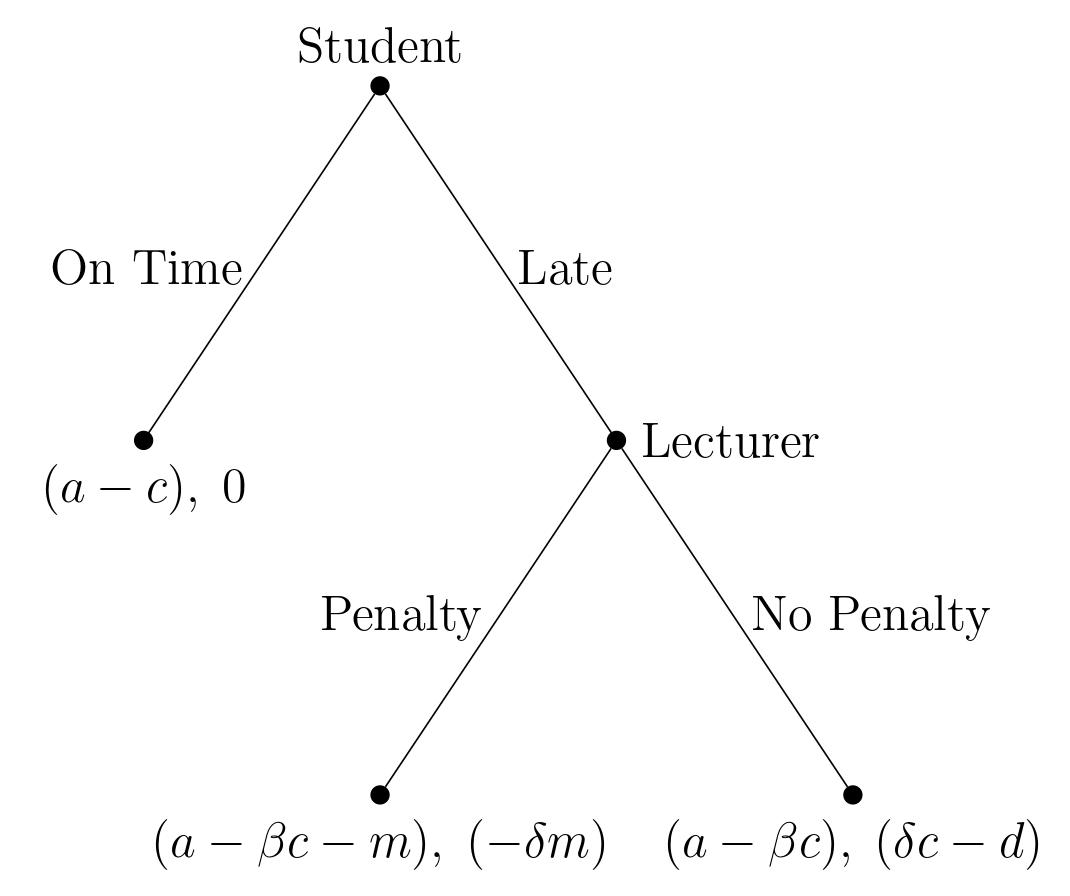
\includegraphics{img/tree} 

}

\caption{Game Tree \label{Figure1}}\label{fig:Figure1}
\end{figure}

\hypertarget{results-and-discussion}{%
\section{\texorpdfstring{Results and Discussion
\label{result}}{Results and Discussion }}\label{results-and-discussion}}

BR interperet Faults with game Run different examples

\begin{table}[H]
\centering
\begin{tabular}{rll}
  \toprule
 & Penalty & No Penalty \\ 
  \midrule
On Time & 0.65, 0 & 0.65, 0 \\ 
  Late & 0.72, -0.01 & 0.77, -0.06 \\ 
   \bottomrule
\end{tabular}
\caption{Simultaneous Game Best Response \label{tab2}} 
\end{table}
\begin{table}[H]
\centering
\begin{tabular}{rll}
  \toprule
 & Student & Lecturer \\ 
  \midrule
Best Response & Late & Penalty \\ 
   \bottomrule
\end{tabular}
\caption{Best Response\label{tab3}} 
\end{table}

\hypertarget{conclusion}{%
\section{\texorpdfstring{Conclusion
\label{con}}{Conclusion }}\label{conclusion}}

Extensions, generality \newpage

\hypertarget{references}{%
\section*{References}\label{references}}
\addcontentsline{toc}{section}{References}

\hypertarget{refs}{}
\begin{CSLReferences}{1}{0}
\leavevmode\hypertarget{ref-harsanyi}{}%
Harsanyi, J.C. 1995. Games with incomplete information. \emph{The
American Economic Review}. 85(3):291--303. {[}Online{]}, Available:
\url{http://www.jstor.org/stable/2118175}.

\leavevmode\hypertarget{ref-book}{}%
Osborne, M.J. 2004. \emph{An introduction to game theory}. Vol. 3. (3).
Oxford university press New York.

\end{CSLReferences}

\newpage

\hypertarget{appendix}{%
\section*{\texorpdfstring{Appendix
\label{app1}}{Appendix }}\label{appendix}}
\addcontentsline{toc}{section}{Appendix \label{app1}}

\hypertarget{payoffs-labelpayoff}{%
\subsection*{Payoffs label\{payoff\}}\label{payoffs-labelpayoff}}
\addcontentsline{toc}{subsection}{Payoffs label\{payoff\}}

\textbf{Student payoffs:} \begin{align*}
E[\text{On Time}]&= a- c \\
E[\text{Late}]&=  p(a-\beta c-m) +(1-p)(a-\beta c) \\
&=-m p+a-\beta c
\end{align*} Student plays on time if: \begin{align*}
a-c>a-m p-\beta c \\
\beta c>c-m p \\
\beta>\frac{c-m p}{c}
\end{align*} Student plays late if: \begin{align*}
\beta<\frac{c-m p}{c}
\end{align*} \textbf{Lecturer Payoffs:} \begin{align*}
E[\text{Penalty}]&=q(-\delta m)+(1-q)(0) \\
&=q(-\delta m) \\
E[\text{No Penalty}] &=q(\delta c-d)+(1-a)(0) \\
&=q(\delta c-d)
\end{align*} Lecturer gives a penalty if: \begin{align*}
q(-\delta m)&>q(\delta c-d) \\
-\delta m&>\delta c-d \\
d&>\delta(c+m) \\
\delta&<\frac{d}{c+m} \\
\delta &<\bar{\delta}
\end{align*} Lecturer gives no penalty if: \begin{align*}
\delta &\geq \frac{d}{c+m} \\
\delta &\geq \bar{\delta} \\
\end{align*}

\hypertarget{best-responses}{%
\subsection*{\texorpdfstring{Best Responses
\label{br}}{Best Responses }}\label{best-responses}}
\addcontentsline{toc}{subsection}{Best Responses \label{br}}

Solving for the best responses: \begin{align*}
p=\text{Probability that the lecturer gives a penalty} = \bar{\delta}=\operatorname{Prob}(\delta<\bar{\delta})
\end{align*} Substitute into the student's best response function -
student hands in on time if: \begin{align*}{}
\beta>\frac{c-m(\bar{\delta})}{c}
\end{align*}{} Since \(0 \leq \beta \leq 1\), \(\beta\) cannot be
greater than 1. This implies \begin{align*}{}
\frac{c-m(\bar{\delta})}{c} \leq 1 \\
c-m \bar{\delta} \leq c \\
-m \bar{\delta} \leq 0 \\
0 \leq \bar{\delta}
\end{align*}{} Since \(0 \leq \bar{\delta} \leq 1\), this condition will
always hold. \(\beta\) cannot be less than 0: \begin{align*}
\frac{c-m \bar{\delta}}{c}&<0 \\
c-m \bar{\delta}&<0 \\
-m \bar{\delta}&< -c \\
\bar{\delta}&>\frac{c}{m}
\end{align*} if \(\bar{\delta}>\frac{c}{m} \Rightarrow \beta=0\),
otherwise: \begin{align*}
\beta =\frac{c-m \bar{\delta}}{c}
\end{align*}

\bibliography{Tex/ref}





\end{document}
